Pour chaque question, recopier sur la copie son numéro et la réponse correspondante.

Pour cette partie, aucune justification n'est demandée.

Pour les questions à choix multiple, une seule réponse est exacte.

\subsection*{Question 1}
Réduire l'expression $A = 4x + 3x$.

\subsection*{Question 2}
Déterminer la médiane de la série statistique suivante : $8$ ; $18$ ; $17$ ; $3$ ; $7$.

\subsection*{Question 3}
Calculer $25\,\%$ de $160$~\euro.

\subsection*{Question 4}
Un triangle est formé d'un angle de $60^{\circ}$ et d'un autre de $100^{\circ}$. Déterminer la mesure, en degré, du troisième angle.

\subsection*{Question 5}
\begin{minipage}{0.63\linewidth}
Recopier sur la copie et compléter par des longueurs des côtés du triangle DEF pour que l'égalité ci-dessous soit vraie :
\[\cos\left(\widehat{\mathrm{DEF}}\right) = \dfrac{\dots}{\dots}\]
\end{minipage}\hfill
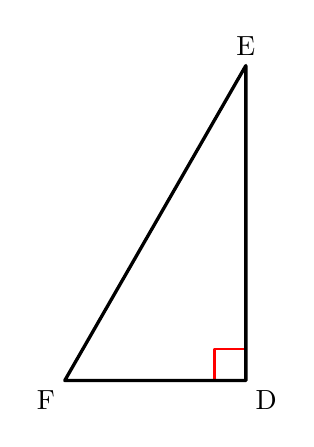
\begin{tikzpicture}[rotate=0,line cap=round, line join=round,baseline={(current bounding box.center)}]
\coordinate (D) at (0,0);
\coordinate (E) at (0,4);
\coordinate (F) at (-2.3,0);
\draw[line width=1pt,red] (0,0) rectangle (-0.4,0.4) ;
\draw[line width=1.2pt] (D) -- (E) -- (F) -- cycle;
\node[below right] at (D) {D};
\node[above] at (E) {E};
\node[below left] at (F) {F};
\end{tikzpicture}

\subsection*{Question 6}
Développer et réduire l'expression $a(3a - 2)$.

\subsection*{Question 7}
Quatre élèves proposent une justification pour montrer que \np{4836} est divisible par 3. Recopier sur la copie le numéro de l'élève qui a justifié correctement.

\begin{center}
\begin{tblr}{*{4}{|X[c]}|}
	\hline
	\textbf{Élève 1} & \textbf{Élève 2} & \textbf{Élève 3} & \textbf{Élève 4} \\
	Le chiffre des unités de \np{4836} est 6, qui est un multiple de 3. & La somme des chiffres de \np{4836} est divisible par 3. & \np{4836} est un nombre pair. & 36 est divisible par 3. \\
	\hline
\end{tblr}
\end{center}

\subsection*{Question 8}
Recopier sur la copie le calcul donnant l'aire, en cm$^2$, d'un disque de diamètre 6 cm.

\begin{center}
\begin{tblr}{*{4}{|X[c]}|}
	\hline
	$\pi \times 6^2$ & $\pi \times 3^2$ & $2 \times \pi \times 3$ & $2 \times \pi \times 6$ \\
	\hline
\end{tblr}
\end{center}

\subsection*{Question 9}
Recopier sur la copie l'expression en fonction de $x$ qui correspond au périmètre du polygone ACDEFB.

\begin{center}
\begin{tikzpicture}[line cap=round, line join=round, scale=0.8]
	\tikzset{
	  singletick/.style={
	    postaction={decorate, decoration={markings,
	      mark=at position 0.5 with {\draw[line width=0.8pt] (0,-0.12)--(0,0.12);}}}
	  },
	  doubletick/.style={
	    postaction={decorate, decoration={markings,
	      mark=at position 0.5 with {
	        \draw[line width=0.8pt] (-0.07,-0.12)--(-0.07,0.12);
	        \draw[line width=0.8pt] ( 0.07,-0.12)--( 0.07,0.12);}}}
	  }
	}
	\coordinate (A) at (0,3);
	\coordinate (B) at (2,1);
	\coordinate (C) at (2.7,3.7);
	\coordinate (D) at (6.7,3.9);
	\coordinate (E) at (7.6,1.1);
	\coordinate (F) at (4.2,-0.3);
	
	% Tracé des segments avec les codages respectifs
	\draw[line width=1.2pt, doubletick] (A) -- (B);
	\draw[line width=1.2pt] (B) -- (F);
	\draw[line width=1.2pt, singletick] (F) -- (E);
	\draw[line width=1.2pt, doubletick] (E) -- (D);
	\draw[line width=1.2pt, singletick] (D) -- (C);
	\draw[line width=1.2pt, doubletick] (C) -- (A);
	\draw[line width=1.2pt, doubletick] (B) -- (C);
	
	% Doubles flèches pour les dimensions (entre la figure et les textes)
	\draw[<->, line width=0.8pt] (-0.2, 2.7) -- (1.8, 0.65);
	\draw[<->, line width=0.8pt] (2.15, 0.5) -- (4.15, -0.7);
	\draw[<->, line width=0.8pt] (4.7, -0.6) -- (7.6, 0.6);
	
	\node[above left] at (A) {A};
	\node[below] at (B) {B};
	\node[above] at (C) {C};
	\node[above] at (D) {D};
	\node[right] at (E) {E};
	\node[below right] at (F) {F};
	\node at (0.5,1.5) {$x$};
	\node at (2.8,-0.3) {3};
	\node at (6.2,-0.30) {4};
\end{tikzpicture}
\end{center}

\begin{center}
\begin{tblr}{*{4}{|X[c]}|}
	\hline
	$4x + 11$ & $x^3 + 11$ & $x + 7$ & $3x + 11$ \\
	\hline
\end{tblr}
\end{center}
